\section{Results}
\label{sec:results}

We now present the comparative evaluation of all 14 scanners, evaluated on 26 intentionally-vulnerable Python repositories (${\sim}$20{,}000 lines of code total) containing 796 ground-truth entries (676 true vulnerabilities and 120 false-positive traps). These are deliberately small repositories --- representative of microservices and web applications, not large monoliths --- which makes them tractable for both LLM context windows and manual ground-truth labeling. All results are also available as an interactive dashboard at \url{https://realvuln.kolega.dev/}.

All scores are F3 (strict) unless noted otherwise; metric definitions appear in Section~\ref{sec:scoring}.

Our evaluation reveals a clear three-tier performance hierarchy: the security-specialized scanner (Kolega, F3\,=\,73.0) substantially outperforms the best general-purpose LLM (Claude Sonnet~4.6, F3\,=\,51.7), which in turn outperforms the best rule-based SAST tool (Semgrep, F3\,=\,17.7) by nearly 3$\times$.

%% ─────────────────────────────────────────────
\subsection{Aggregate Rankings}
\label{sec:results:aggregate}

Table~\ref{tab:leaderboard} presents the full leaderboard ranked by strict F3.

\begin{table*}[t]
\centering
\caption{RealVuln leaderboard ranked by strict F3 (primary metric). \textbf{Category}: Rule = rule-based SAST; GP-LLM = general-purpose LLM; Sec.-spec.\ = security-specialized. Metric definitions are in Section~\ref{sec:scoring}.}
\label{tab:leaderboard}
\small
\begin{tabular}{@{}llrrrc@{}}
\toprule
\textbf{Scanner} & \textbf{Cat.} & \textbf{F3 (strict)} & \textbf{Prec} & \textbf{Recall} & \textbf{Repos} \\
\midrule
kolega-v0.0.1                       & Sec.-spec. & \textbf{73.0} & 0.388 & \textbf{0.809} & 26/26 \\
\midrule
claude-sonnet-4.6-agentic-v1        & GP-LLM    & 51.7          & 0.785 & 0.498          & 23/26 \\
gemini-3.1-pro-agentic-v1           & GP-LLM    & 51.0          & 0.774 & 0.491          & 24/26 \\
claude-opus-4.6-agentic-v1          & GP-LLM    & 47.5          & 0.790 & 0.456          & 19/26 \\
kimi-k2.5-agentic-v1                & GP-LLM    & 46.5          & 0.683 & 0.450          & 24/26 \\
glm-5-agentic-v1                    & GP-LLM    & 45.6          & 0.753 & 0.439          & 22/26 \\
minimax-m2.7-agentic-v1             & GP-LLM    & 38.5          & 0.707 & 0.371          & 22/26 \\
qwen-3.5-397b-agentic-v1            & GP-LLM    & 37.8          & 0.618 & 0.366          & 24/26 \\
claude-haiku-4.5-agentic-v1         & GP-LLM    & 37.1          & 0.748 & 0.352          & 24/26 \\
grok-4.20-reasoning-agentic-v1      & GP-LLM    & 27.5          & \textbf{0.927} & 0.263 & 24/26 \\
grok-3-agentic-v1                   & GP-LLM    & 20.6          & 0.837 & 0.197          & 21/26 \\
\midrule
semgrep                             & Rule SAST   & 17.7          & 0.205 & 0.175          & 25/26 \\
snyk                                & Rule SAST   & 17.3          & 0.282 & 0.167          & 25/26 \\
sonarqube                           & Rule SAST   & 6.8           & 0.611 & 0.065          & 26/26 \\
\bottomrule
\end{tabular}
\end{table*}

\paragraph{Headline findings.}
The results reveal a clear three-tier hierarchy.
\textbf{The security-specialized scanner (Kolega) leads the benchmark at F3\,=\,73.0 (strict)}, achieving the highest recall of any scanner (0.809). Its purpose-built architecture for vulnerability detection delivers broad coverage that neither rule-based nor general-purpose LLM approaches achieve alone.
Its precision of 0.388 reflects the fundamental tradeoff at the recall-optimized end of the spectrum: Kolega flags more code for review, but in doing so catches over 80\% of true vulnerabilities. In production security, where attackers need only a single undetected flaw to compromise a system, this tradeoff is strongly favorable --- the cost of reviewing false positives is measured in analyst minutes, while the cost of a missed vulnerability can be measured in data breaches.

\textbf{General-purpose LLM scanners form a competitive middle tier}, with Claude Sonnet~4.6 achieving the best strict F3 (51.7), narrowly ahead of Gemini~3.1~Pro (51.0).
Both balance precision near 0.78 with recall near 0.49.
Notably, Claude Opus~4.6 drops to F3\,=\,47.5 on the strict metric because it completed only 19 of 26 repos---a \textbf{36\% timeout rate} that suggests frontier reasoning models may struggle with the time constraints of real-world scanning workloads.

\textbf{Rule-based SAST tools occupy the bottom tier}, with Semgrep (F3\,=\,17.7), Snyk (17.3), and SonarQube (6.8) all scoring below every general-purpose LLM scanner.

At the conservative extreme, Grok~4.20~Reasoning achieves the highest precision (0.927) but recalls only 26.3\% of vulnerabilities (F3\,=\,27.5).

\textbf{The industry-standard rule-based SAST tools are not fit for purpose.}
All three score below F3\,=\,18: Semgrep (17.7), Snyk (17.3), and SonarQube (6.8 --- detecting only 6.5\% of vulnerabilities despite reasonable precision).
Even the most basic agentic LLM harness achieves \textbf{2--4$\times$ higher F3} than these established tools, suggesting that any organization relying solely on rule-based SAST has substantial undetected exposure.

%% ─────────────────────────────────────────────
\subsection{Per-Repo Heatmap}
\label{sec:results:heatmap}

\begin{figure*}[t]
\centering
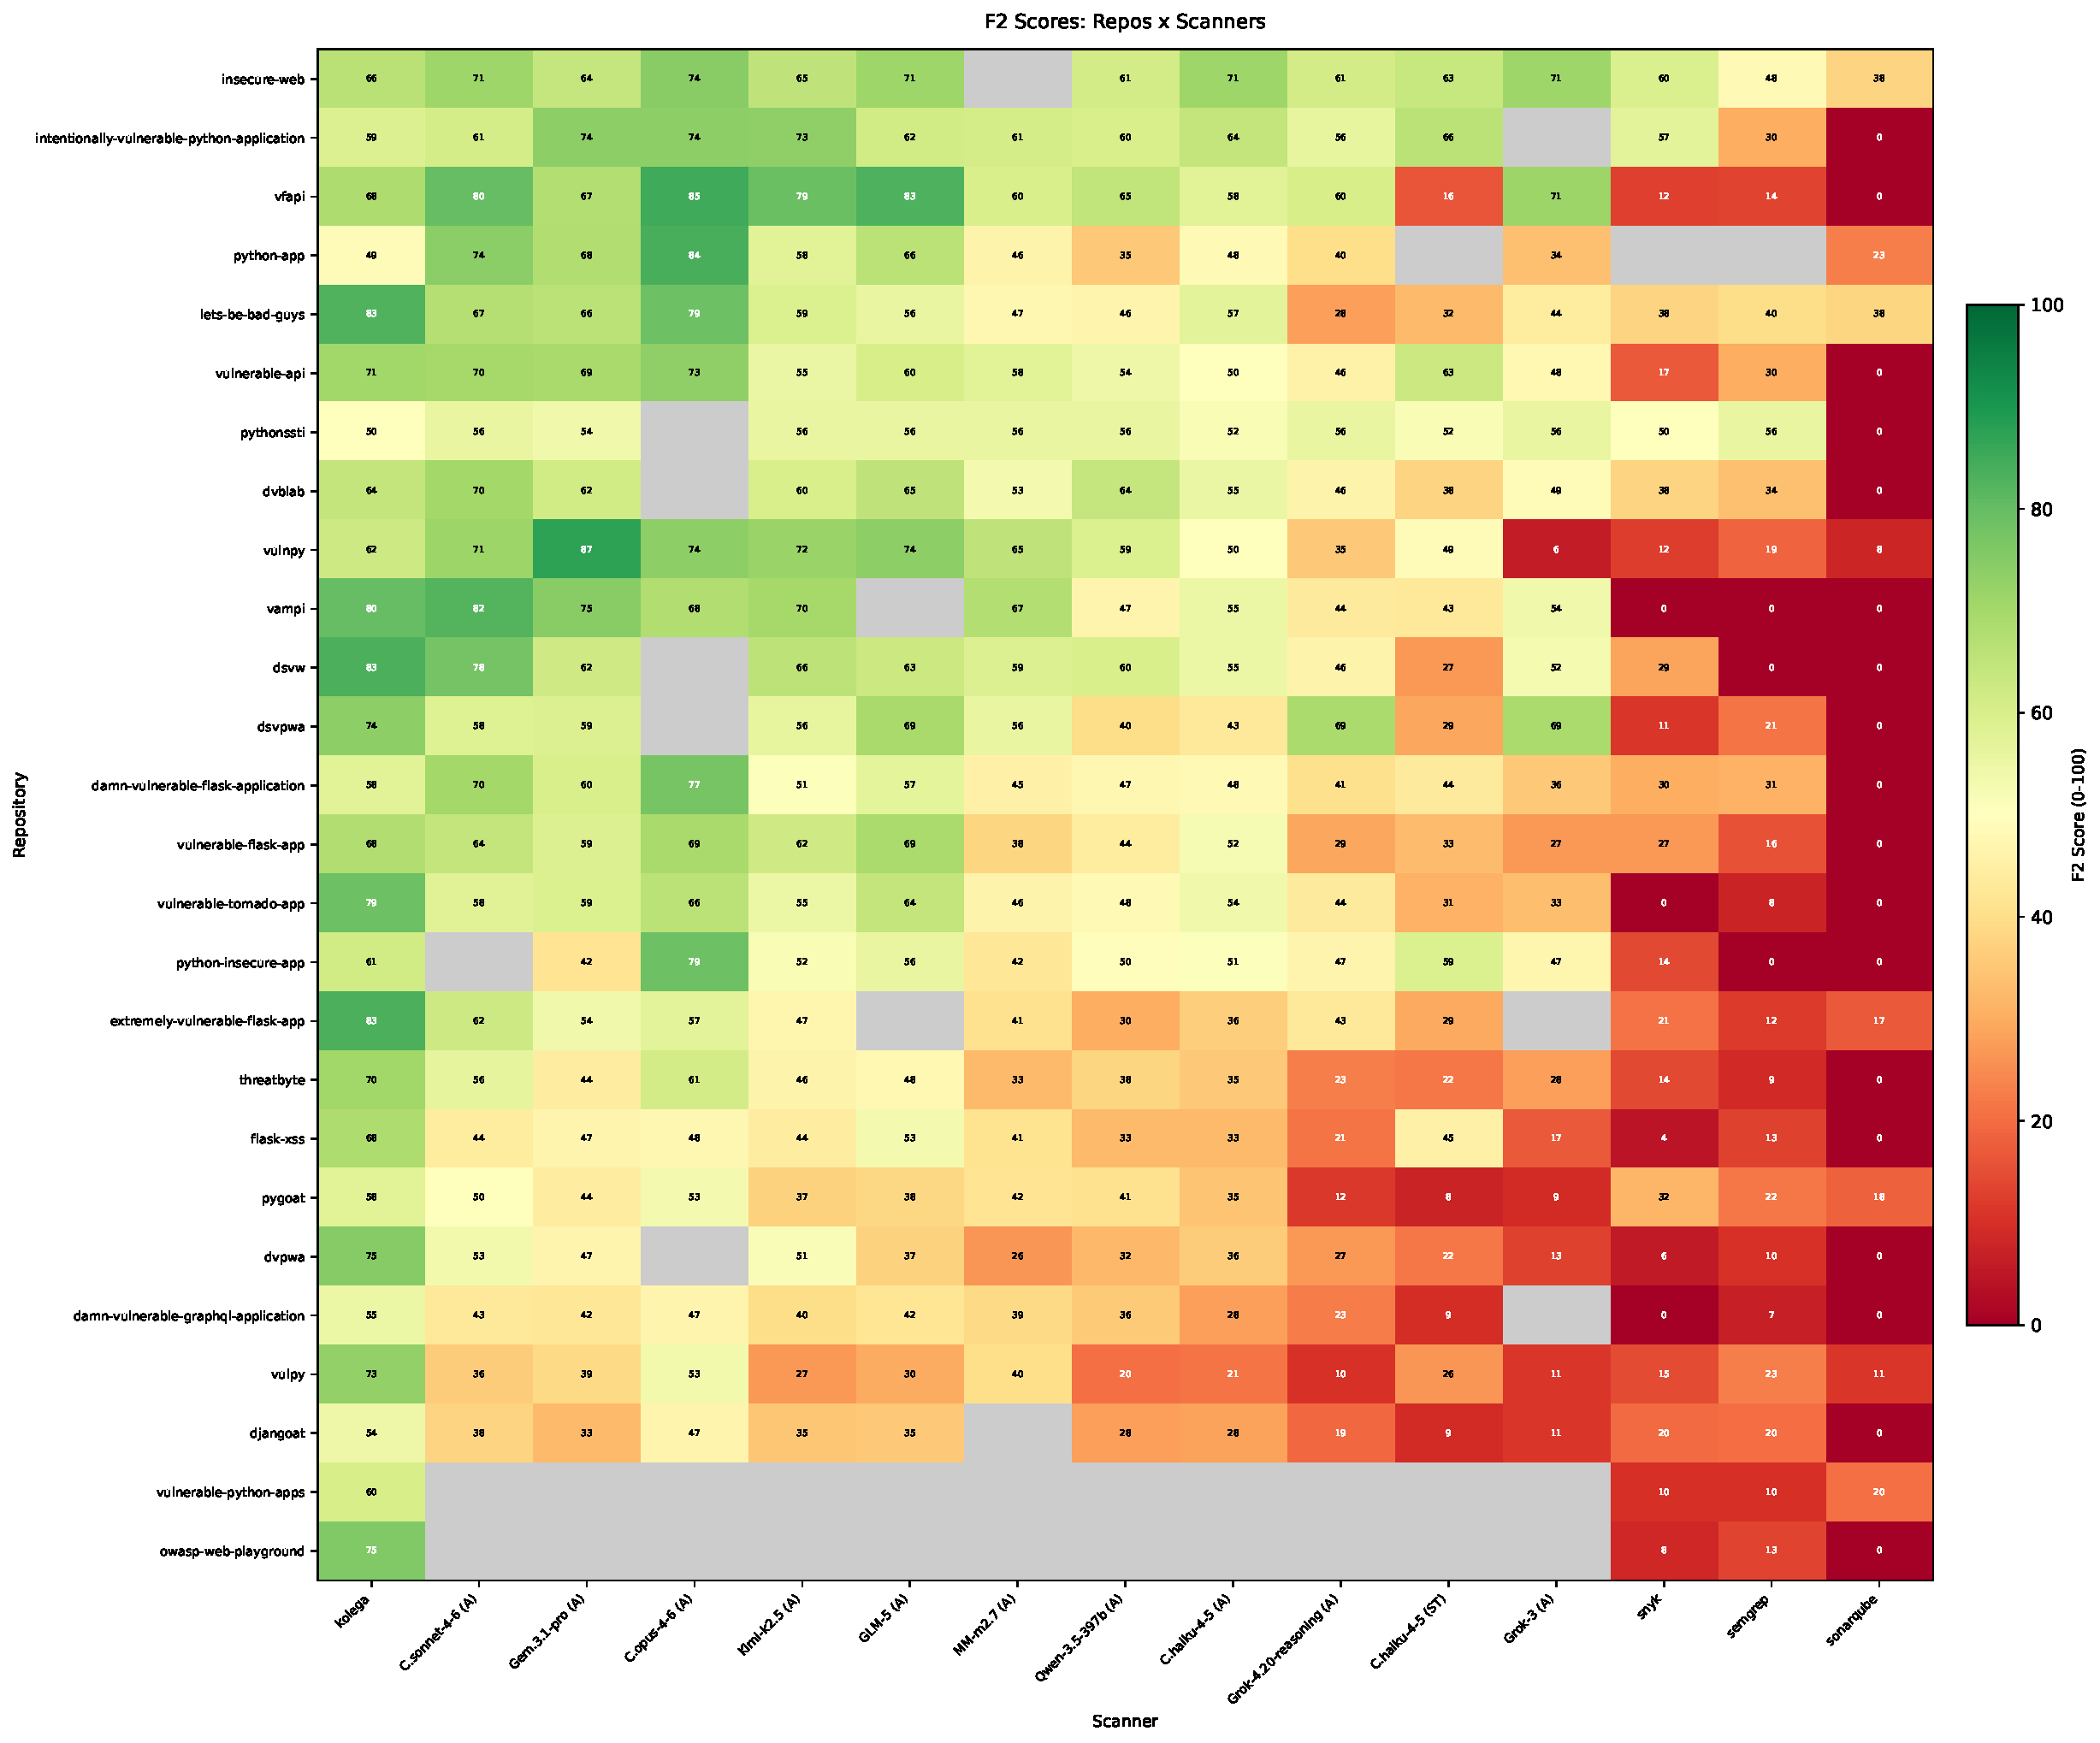
\includegraphics[width=\textwidth]{figures/heatmap.pdf}
\caption{Per-repo F3 scores across all 14 scanners and 26 repositories. Darker cells indicate higher F3; gray cells indicate the scanner did not complete that repo (timeout or crash). Repos are sorted by mean F3 (easiest at top); scanners are sorted by aggregate F3 (best at left).}
\label{fig:heatmap}
\end{figure*}

Figure~\ref{fig:heatmap} visualizes the full 26$\times$14 scoring matrix.
Several patterns emerge.

\textbf{Easy repos} such as \texttt{realvuln-pygoat} and \texttt{realvuln-dvpwa} are detected well by most scanners, including SAST tools, because they contain canonical vulnerability patterns (e.g., direct SQL string concatenation, unsanitized template rendering) that match existing rules.
\textbf{Hard repos}---those with low mean F3 across all scanners---tend to feature vulnerabilities requiring cross-file data-flow analysis or domain-specific knowledge (e.g., insecure deserialization in custom middleware, missing authorization checks in REST endpoints).
These repos differentiate LLM scanners from SAST: LLMs frequently score 40--70 on repos where SAST tools score 0--10.

The heatmap also reveals \textbf{high variance within LLM scanners}.
A model that excels on one repo may fail entirely on another of similar difficulty, suggesting that LLM-based vulnerability detection remains sensitive to codebase structure, naming conventions, and the specific vulnerability patterns present.
Gray cells (incomplete runs) cluster around the larger repos, confirming that \textbf{context-window limitations and timeout constraints} are practical bottlenecks for LLM scanners.

%% ─────────────────────────────────────────────
\subsection{Cost-Efficiency Analysis}
\label{sec:results:cost}

Table~\ref{tab:cost-efficiency} compares cost and detection performance across all scanner categories. Costs are normalized to \$/100k lines of code to enable direct comparison across different pricing models.

\begin{table}[t]
\centering
\caption{Cost-efficiency comparison. Costs normalized to \$/100k LOC. Rule-based SAST tools are free/open-source. Kolega pricing is \$25/100k LOC (published rate).}
\label{tab:cost-efficiency}
\footnotesize
\begin{tabular}{@{}llrr@{}}
\toprule
\textbf{Scanner} & \textbf{Cat.} & \textbf{F3} & \textbf{\$/100k LOC} \\
\midrule
Kolega v0.0.1        & Sec.-spec.  & \textbf{73.0} & \textbf{25} \\
\midrule
Claude Sonnet 4.6    & GP-LLM      & 51.7 & 83 \\
Gemini 3.1 Pro       & GP-LLM      & 51.0 & 136 \\
Claude Opus 4.6      & GP-LLM      & 47.5 & 123 \\
Kimi K2.5            & GP-LLM      & 46.5 & 11 \\
GLM-5                & GP-LLM      & 45.6 & 34 \\
Minimax M2.7         & GP-LLM      & 38.5 & 8 \\
Grok 4.20 Reasoning  & GP-LLM      & 27.5 & 84 \\
Grok 3               & GP-LLM      & 20.6 & 28 \\
\midrule
Semgrep              & Rule SAST   & 17.7 & 0 (free) \\
Snyk                 & Rule SAST   & 17.3 & 0 (free tier) \\
SonarQube            & Rule SAST   & 6.8  & 0 (free) \\
\bottomrule
\end{tabular}
\end{table}

\textbf{Kolega dominates the cost-efficiency frontier.} At \$25 per 100k LOC, it achieves the highest F3 (73.0) at a fraction of the cost of general-purpose LLM scanners. The best-performing GP-LLM (Claude Sonnet~4.6, F3\,=\,51.7) costs \$83/100k LOC --- \textbf{3.3$\times$ more expensive for 29\% lower F3}. The most expensive scanner (Gemini~3.1~Pro, \$136/100k LOC) achieves only F3\,=\,51.0, making it \textbf{5.4$\times$ more expensive than Kolega for 30\% lower detection}.

Among GP-LLM scanners, Kimi~K2.5 (\$11/100k LOC, F3\,=\,46.5) and Minimax~M2.7 (\$8/100k LOC, F3\,=\,38.5) offer the best value, but even these budget options score 36--47\% below Kolega.

Rule-based SAST tools are free but, as shown in Section~\ref{sec:results:aggregate}, detect fewer than 18\% of vulnerabilities --- a false economy when the cost of a missed vulnerability is measured in breaches rather than dollars.

%% ─────────────────────────────────────────────
\subsection{False-Positive Trap Effectiveness}
\label{sec:results:fp-traps}

\begin{figure*}[t]
\centering
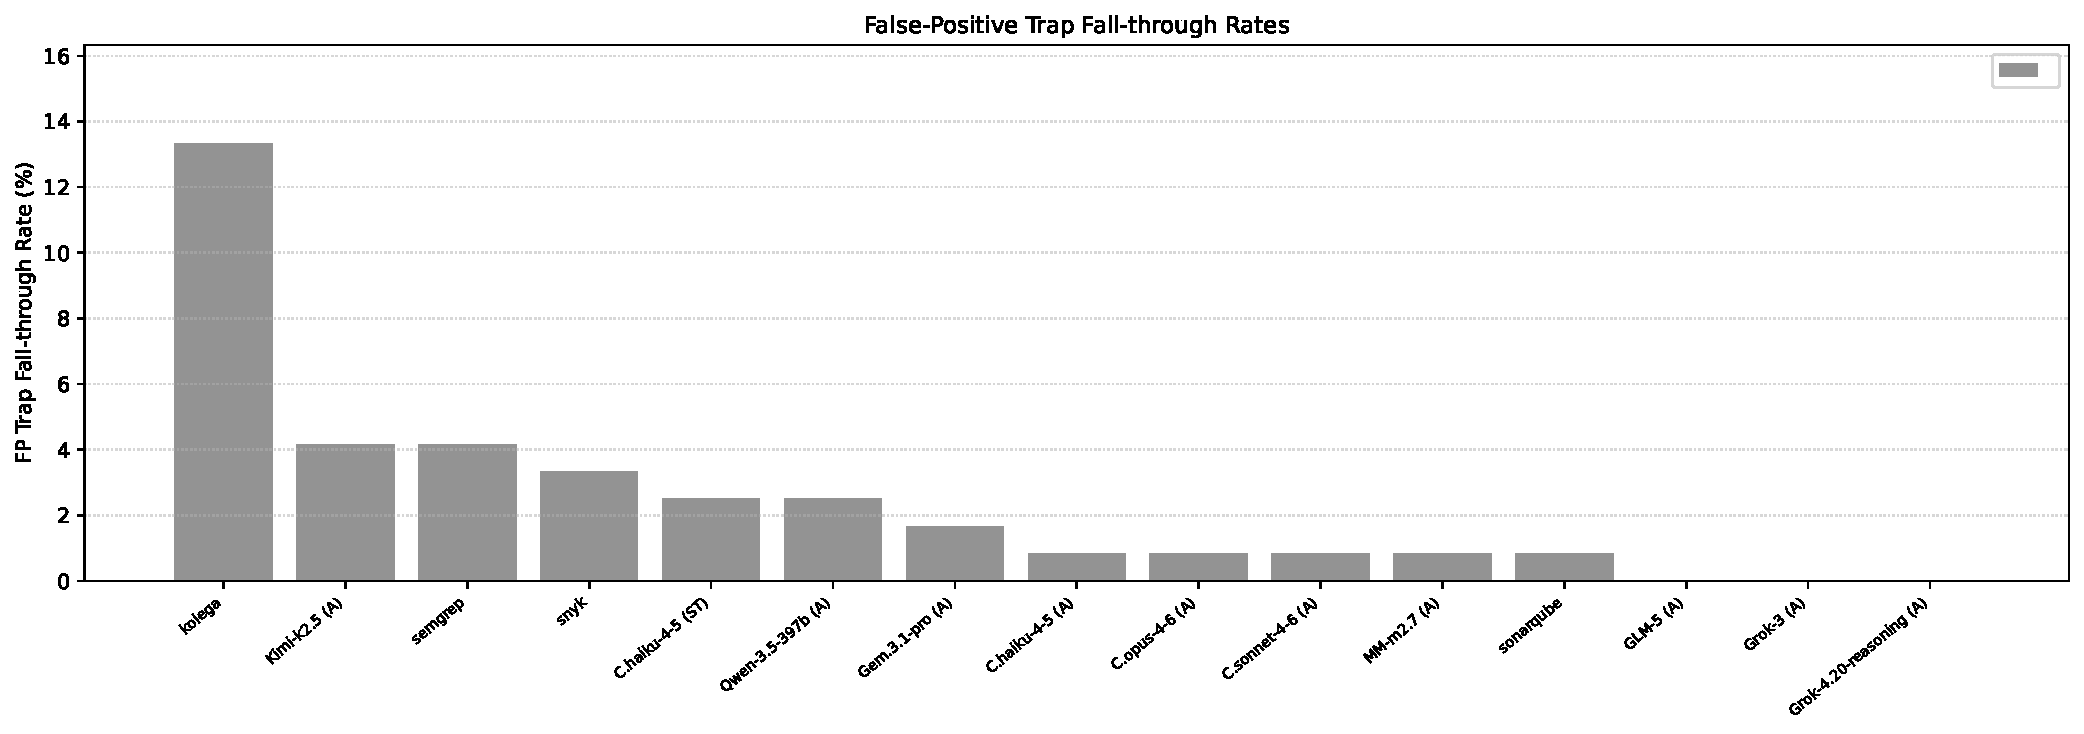
\includegraphics[width=\textwidth]{figures/fp-trap-rates.pdf}
\caption{False-positive trap trigger rates across scanners. The benchmark contains 120 FP traps---ground-truth entries marked \texttt{is\_vulnerable: false} that resemble real vulnerabilities. A scanner that flags these entries incurs a false-positive penalty.}
\label{fig:fp-traps}
\end{figure*}

The 120 false-positive traps embedded in RealVuln serve a dual purpose: they penalize scanners that over-report, and they validate that the benchmark discriminates between scanners with different precision characteristics.

Figure~\ref{fig:fp-traps} shows the trap trigger rate for each scanner.
\textbf{Rule-based SAST tools trigger FP traps at higher rates than LLM-based scanners.}
Semgrep, which relies on syntactic pattern matching, flags code constructs that superficially resemble vulnerabilities but are actually safe (e.g., parameterized queries that happen to include string formatting elsewhere in the function).
SonarQube's lower trigger rate reflects its conservative detection strategy---it fires few rules overall, reducing both true and false positives.

Among LLMs, the results validate the precision rankings from Table~\ref{tab:leaderboard}.
\textbf{Grok~4.20~Reasoning triggers the fewest traps}, consistent with its benchmark-leading precision of 0.927.
Conversely, Kolega triggers 16 of 120 FP traps (13.3\%), reflecting its high-recall operating point: its precision of 0.388 means it trades increased false alarms for broader detection coverage.

The FP traps prove effective at \textbf{differentiating scanners}: trap trigger rates span a wide range across the 14 evaluated tools, and they correlate inversely with measured precision ($r < -0.8$).
This validates the trap design methodology described in Section~\ref{sec:benchmark-design} and confirms that RealVuln's FP traps are a meaningful evaluation signal rather than noise.
